\documentclass[11pt]{article}
\usepackage{graphicx}
\usepackage[margin=1in]{geometry} %reducir márgenes
\usepackage{cite} %opciones entre {}
\pagestyle{empty} %quitar números de página

\parindent 0ex 
\renewcommand{\baselinestretch}{1.2} 

\begin{document}

\section*{\textbf{Cambios Sprints \& Milestones} } %definir estilo de la función
Desde la página de support de zenhub escribieron un articulo con una comparación entre\textit{Milestones vs. Releases}. Se plantea como organizar la información \textit{Epic} o \textit{Milestone} o como un \textit{Releases}.\\

GitHub Milestones estan destinados a equipos con iteraciones cortas y un alcance limitado a ningún cambio (Además GitHub Milestones usa el Gráfico Burndown, indicando el estado de las issues completado, abierto e incompleto dentro de ese Sprint, estas ultimas se terminaran en proximos Sprints). Por otra parte, tenemos Zenhub Releases que esta más destinado a proyectos de larga duración, permitiendo cambios.\\

También desde el Zenhub han dado información sobre los cambios de cara a final de año, GitHub Miles7tone no aparecera proximante desde ZenHub, según comentan la mayoría de equipos de trabajo ya se habrían cambiado a los Sprints Automáticos. A continuación resumiremos algunos consejos que nos han dado para familiarizarnos con esta nueva forma de trabajar.\\

El objetivo de esta implentación es reducir los tiempos que dedican los equipos de trabajo en construir la ruta de trabajo. Para ello han automatizado tareas como crear sprints, añadir issues, mover issues no terminadas al siguiente sprint y una mayor visibilidad del alcance del sprint("sprint scope").\\

En cuanto a la creación de estos Sprints Automáticos. Creando un Sprint con una fecha de comienzo y una de fin, se crean automáticamente dos sprints más, basados en la duración que hayamos asignado a este primero. De esta forma aligeramos mucho el proceso de gestión de sprint al estar ya propuesta una duración de los mismos. \cite{Sprint_planning}\\

%configurar opcion entre parrafos dejar una linea

La figura \ref{fig:sprints} podemos ver como al generar un sprint (color azul) génera otros dos más abajo dejando libres los mismos días que habiamos decidido excluir en las dos semanas de trabajo.

\begin{figure}[h!] %PARA QUE SE QUEDE EN ESTA ZONA DEL TEXTO
\centering
    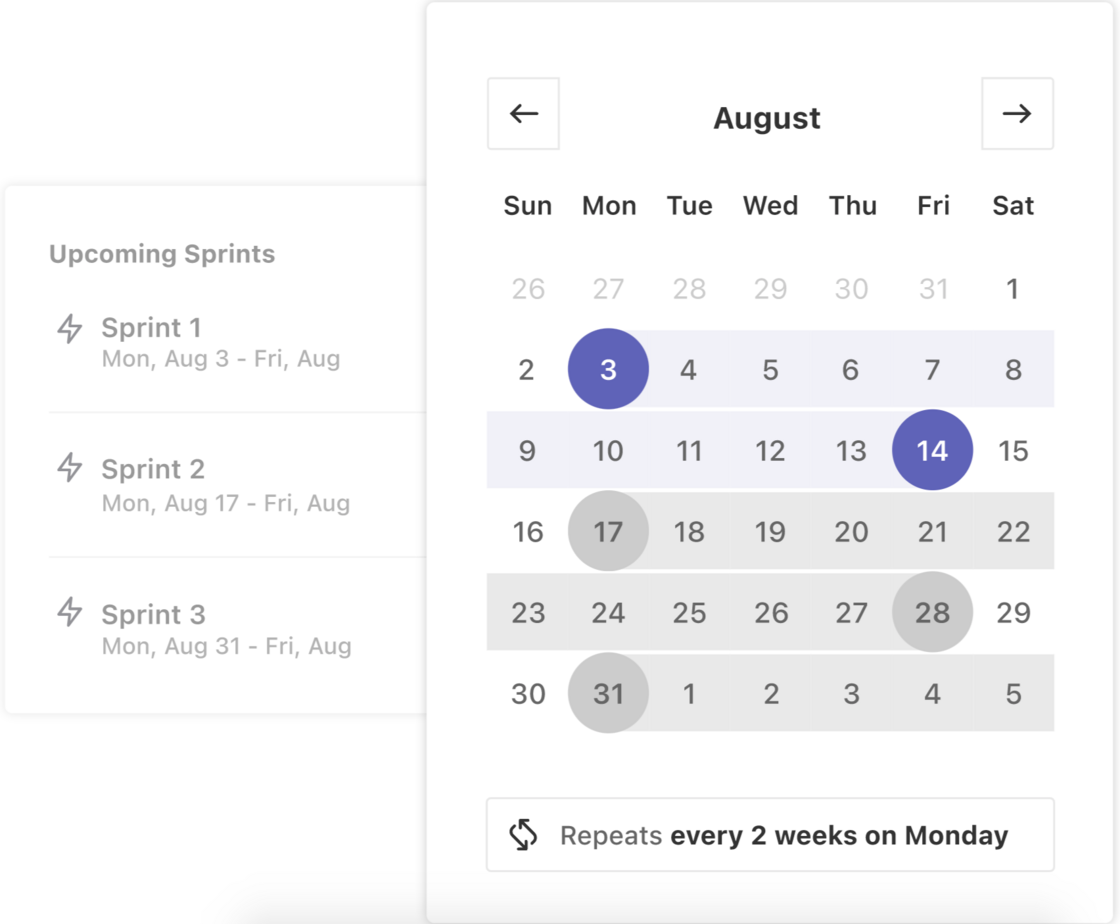
\includegraphics[width=0.4\textwidth]{sprints_automaticas}
\caption{Creación Sprints Automáticos}
\label{fig:sprints}
\end{figure}

Actualmente las issues solo pueden pertener a un \textit{GitHub Milestone} a la vez. Esto hace que si no está terminada en un mismo \textit{milestone}, tiene que ser borrada y creada en el próximo \textit{milestone}(Se pierde información al tenerse que crear y completar en  un mismo milestone). Con estos últimos cambios las issues pueden encontrarse en multiples Sprints al mismo tiempo. Ofrecinedonos opciones como mover las issues incompletas al siguietne sprint.








%bibliografia diferencia con references

\bibliographystyle{plain}
\bibliography{library}


\end{document}